\begin{figure}[ht]
  \centering
  \begin{subfigure}{.49\textwidth}
    \centering
    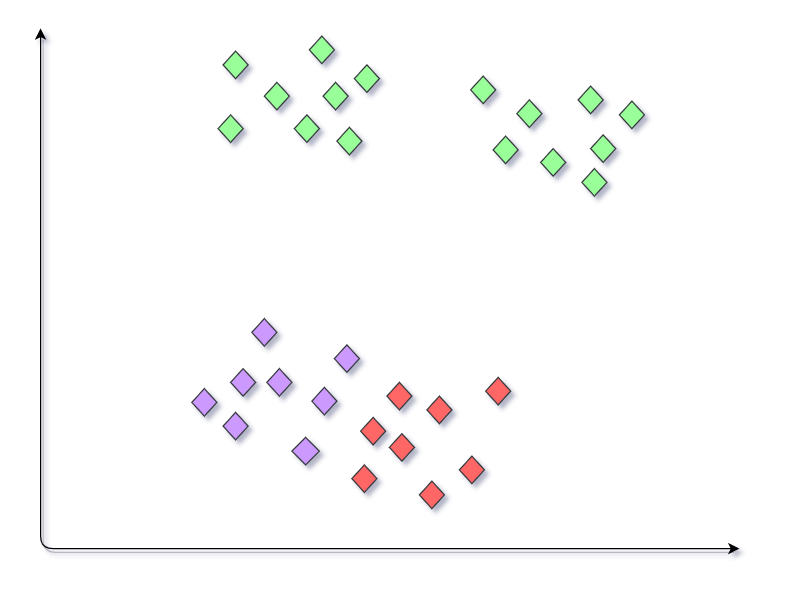
\includegraphics[width=.9\linewidth]{./Chapitre2/figures/kmeans1.png}
  \end{subfigure}
  \begin{subfigure}{.49\textwidth}
    \centering
    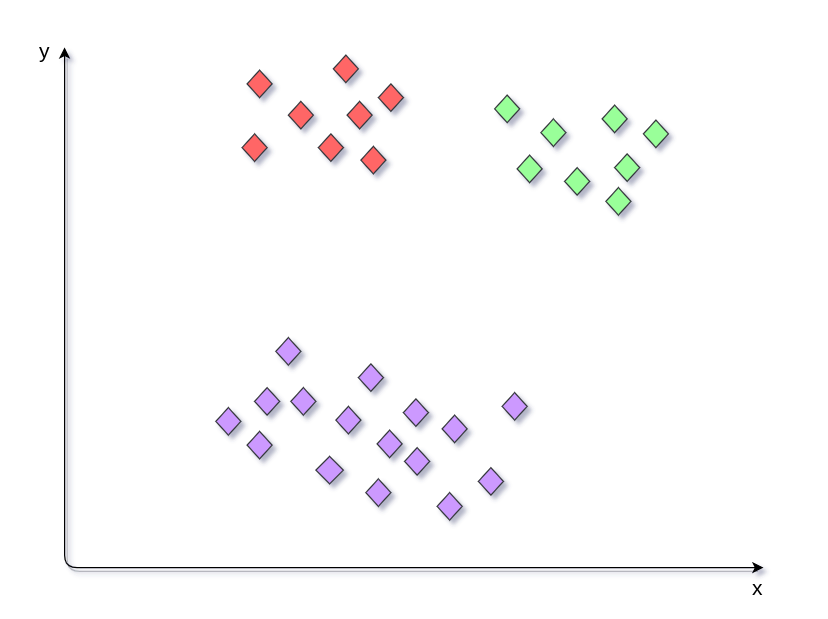
\includegraphics[width=.9\linewidth]{./Chapitre2/figures/kmeans2.png}
  \end{subfigure}
  \caption{Deux classifications en 3 classes utilisant l'algorithme k-moyennes avec deux initialisations de centroides différentes. Ici les données sont des points de coordonnées $(x,y)$. Illustrations issues de shorturl.at/htMN6 .}
  \label{fig:kmeans}
\end{figure}
